%-------------------------
% Two-Page Professional Resume
% Author: Milav Jayeshkumar Dabgar
% Compiled with XeLaTeX for best results
%-------------------------

\documentclass[11pt,a4paper]{article}

% Packages for XeLaTeX
\usepackage{fontspec}
\usepackage{xunicode}
\usepackage{xltxtra}

% Modern fonts
\setmainfont{Liberation Serif}[Scale=1.0]
\setsansfont{Liberation Sans}[Scale=1.0]
\setmonofont{Liberation Mono}[Scale=1.0]

% Packages
\usepackage[top=0.6in, bottom=0.6in, left=0.6in, right=0.6in]{geometry}
\usepackage{xcolor}
\usepackage{titlesec}
\usepackage{enumitem}
\usepackage{multicol}
\usepackage{fontawesome5}
\usepackage{hyperref}
\usepackage{tikz}
\usepackage{array}
\usepackage{tabularx}

% Colors
\definecolor{primary}{RGB}{0, 79, 144}
\definecolor{secondary}{RGB}{45, 45, 45}
\definecolor{lightgray}{RGB}{248, 248, 248}
\definecolor{mediumgray}{RGB}{128, 128, 128}

% Hyperref setup
\hypersetup{
    colorlinks=true,
    linkcolor=primary,
    urlcolor=primary,
    pdfauthor={Milav Jayeshkumar Dabgar},
    pdftitle={Resume - Milav Jayeshkumar Dabgar - Two Page},
    pdfsubject={Professional Resume},
    pdfkeywords={AICTE Fellowship, AI, Data Science, Engineering Education, Innovation, R&D}
}

% Remove page numbers
\pagestyle{empty}

% Custom section formatting
\titleformat{\section}
    {\color{primary}\Large\sffamily\bfseries}
    {}
    {0em}
    {}[{\color{primary}\titlerule[1pt]\vspace{-2pt}}]

% Improved spacing
\titlespacing*{\section}{0pt}{10pt}{6pt}

% Custom commands
\newcommand{\resumeItem}[1]{
    \item\small{#1 \vspace{-1pt}}
}

\newcommand{\resumeSubheading}[4]{
    \vspace{-1pt}\item
    \begin{tabular*}{0.97\textwidth}[t]{l@{\extracolsep{\fill}}r}
        \textbf{\small\color{secondary}#1} & \textbf{\color{mediumgray}\small #2} \\
        \textit{\small\color{primary}#3} & \textit{\small\color{mediumgray} #4} \\
    \end{tabular*}\vspace{-2pt}
}

\newcommand{\resumeProjectHeading}[2]{
    \vspace{-1pt}\item
    \begin{tabular*}{0.97\textwidth}{l@{\extracolsep{\fill}}r}
        \small\textbf{\color{secondary}#1} & \textbf{\color{mediumgray}\small #2} \\
    \end{tabular*}\vspace{-2pt}
}

\newcommand{\resumeSubHeadingListStart}{\begin{itemize}[leftmargin=0.15in, label={}]}
\newcommand{\resumeSubHeadingListEnd}{\end{itemize}}
\newcommand{\resumeItemListStart}{\begin{itemize}[leftmargin=0.25in]}
\newcommand{\resumeItemListEnd}{\end{itemize}\vspace{-3pt}}

% Enhanced header design (simplified for two-page)
\newcommand{\makeheader}{
    \begin{center}
        \begin{tikzpicture}[remember picture, overlay]
            \fill[lightgray] (current page.north west) rectangle ([yshift=-2.5cm]current page.north east);
        \end{tikzpicture}
        
        \vspace{0.2cm}
        \begin{minipage}[t]{0.75\textwidth}
            \raggedright
            {\huge\sffamily\bfseries\color{primary} Milav Jayeshkumar Dabgar}
            
            \vspace{4pt}
            {\large\sffamily\color{secondary} Engineering Educator \& R\&D Professional}
            
            \vspace{6pt}
            {\small\color{secondary} Innovation Leader $\bullet$ Full-Stack Developer $\bullet$ AI/Data Science Practitioner}
            
            \vspace{8pt}
            \small
            \faIcon{envelope}\,\href{mailto:milav.dabgar@gmail.com}{\color{primary}milav.dabgar@gmail.com} $\bullet$
            \faIcon{phone}\,+91 8128576285 $\bullet$
            \faIcon{linkedin}\,\href{https://linkedin.com/in/milavdabgar}{\color{primary}linkedin.com/in/milavdabgar} \\
            \vspace{2pt}
            \faIcon{github}\,\href{https://github.com/milavdabgar}{\color{primary}github.com/milavdabgar} $\bullet$
            \faIcon{globe}\,\href{https://milav.in}{\color{primary}milav.in} $\bullet$
            \color{mediumgray}Gujarat, India $\bullet$ AICTE ID: 1-3241967546
        \end{minipage}
        \hfill
        \begin{minipage}[t]{0.2\textwidth}
            \raggedleft
            \vspace{0.1cm}
            \begin{tikzpicture}
                \clip (0,0) circle (1.2cm);
                \node at (0,0) {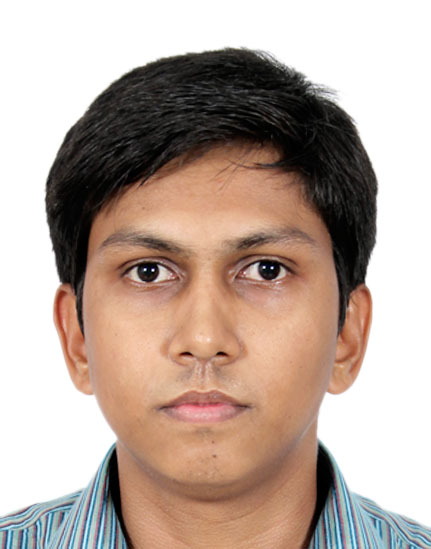
\includegraphics[width=2.4cm, height=2.4cm, keepaspectratio]{profile-picture.jpg}};
                \draw[primary, line width=2pt] (0,0) circle (1.2cm);
            \end{tikzpicture}
        \end{minipage}
    \end{center}
    \vspace{0.2cm}
}

%-------------------------------------------
%%%%%%  RESUME STARTS HERE  %%%%%%%%%%%%%%%%%%%%%%%%%%%%
%-------------------------------------------

\begin{document}

\makeheader

%----------- EXECUTIVE SUMMARY -----------
\section{Executive Summary}
\small
Engineering educator and R\&D professional with \textbf{9+ years} of comprehensive experience spanning electronics hardware development, embedded systems, AI/ML, and full-stack software engineering. Currently pursuing \textbf{BS in Data Science and Applications from IIT Madras} (Diploma in Programming completed with distinction). Distinguished by exceptional student mentorship that enabled teams to secure \textbf{Rs. 45+ lakhs in innovation funding} (Rs. 25 lakhs from Shark Tank India, Rs. 20 lakhs from iHub Gujarat), resulting in \textbf{2 student patents}. Proven expertise in bridging academia-industry gap through innovative teaching methodologies, self-hosted infrastructure development, and real-world system implementation. Seeking AICTE Industry Fellowship to gain advanced industrial research experience and enhance diploma-level innovation ecosystem in Gujarat.

%----------- PROFESSIONAL EXPERIENCE -----------
\section{Professional Experience}
\resumeSubHeadingListStart

\resumeSubheading
{Lecturer (Class - II) \& Innovation Leader}{Nov 2016 -- Present}
{Government Polytechnic, Education Department - Government of Gujarat}{Palanpur, Gujarat}
\resumeItemListStart
\resumeItem{Lead comprehensive technical education across Programming in C, Microprocessor Programming, Embedded Systems, Circuit Design, Consumer Electronics, and Entrepreneurship}
\resumeItem{Hold key institutional positions: \textbf{IT Convener} (infrastructure strategy), \textbf{SSIP Co-Convener} (startup ecosystem), \textbf{Training \& Placement Member}, and active contributor to MIS and UDAYAM initiatives}
\resumeItem{Achieved remarkable student success: mentored teams securing \textbf{Rs. 25 lakhs from Shark Tank India} and \textbf{Rs. 20 lakhs through government innovation programs}, resulting in \textbf{2 student patents}}
\resumeItem{Architected and deployed comprehensive \textbf{Next.js Academic Management System} at \href{https://gppalanpur.in/}{gppalanpur.in} with production-grade CI/CD pipeline, featuring complete institutional management with CSV import/export, advanced search/filter/sort capabilities, and automated feedback analysis}
\resumeItem{Developed student portfolio system with LinkedIn-style public profiles, downloadable biodata/resume/CV generation, interactive newsletters with PDF/HTML export, and comprehensive paper solutions for ECE/ICT/IT branches in English/Gujarati}
\resumeItem{Designed enterprise-grade infrastructure: self-hosted Linux servers, Dockerized microservices, CI/CD pipelines, and automated backup systems}
\resumeItemListEnd

\resumeSubheading
{Electronics \& Communication Engineer (R\&D)}{Jul 2015 -- Oct 2016}
{TEXEG India Private Limited (Japan-based Technology Firm)}{Gandhinagar, Gujarat}
\resumeItemListStart
\resumeItem{Led end-to-end product development lifecycle for commercial embedded systems in international R\&D environment}
\resumeItem{Executed circuit simulation, PCB design, firmware development, and control systems implementation}
\resumeItem{Designed control algorithms (PID, PI, Fuzzy Logic) using MATLAB Control System Toolbox for industrial applications}
\resumeItem{Delivered complete embedded solutions from concept to production, supporting cross-functional mechanical engineering teams}
\resumeItemListEnd

\resumeSubheading
{Research \& Development Intern}{Aug 2014 -- Jul 2015}
{eiTRA - eInfochips Training \& Research Academy Ltd}{Ahmedabad, Gujarat}
\resumeItemListStart
\resumeItem{Gained comprehensive foundation in embedded systems research methodologies and industry best practices}
\resumeItem{Developed proficiency in advanced debugging techniques and hardware-software integration strategies}
\resumeItemListEnd

\resumeSubHeadingListEnd

%----------- EDUCATION -----------
\section{Education}
\resumeSubHeadingListStart

\resumeSubheading
{Bachelor of Science (BS) in Data Science and Applications}{2021 -- Present}
{Indian Institute of Technology Madras (IIT Madras)}{Roll No: 21F1005510 | Overall CGPA: 7.07/10}
\resumeItemListStart
\resumeItem{\textbf{Foundation Level:} Completed (32/32 credits, CGPA: 7.50/10) - Strong performance in Computational Thinking, Mathematics for Data Science, and Programming in Python}
\resumeItem{\textbf{Diploma Programming Track:} Completed (27/27 credits, CGPA: 7.19/10) - Database Management, Data Structures \& Algorithms, Modern Application Development I \& II with project work}
\resumeItem{\textbf{Diploma Data Science Track:} In Progress (21/27 credits, CGPA: 6.24/10) - Machine Learning Techniques, Business Analytics, Business Data Management}
\resumeItem{\textbf{Current Status:} 80/142 credits completed toward full degree | Final phase coursework in Machine Learning Practice and Business Data Management projects}
\resumeItemListEnd

\resumeSubheading
{Master of Engineering(ME), Communication Systems}{2013 -- 2015}
{L.D College of Engineering, Gujarat Technological University}{Ahmedabad, Gujarat | CGPA: 8.04/10}
\resumeItemListStart
\resumeItem{Specialized in Digital Signal Processing, Wireless Communications, and Advanced Communication Protocols}
\resumeItemListEnd

\resumeSubheading
{Bachelor of Engineering(BE), Electronics \& Communication}{2009 -- 2013}
{Sal Institute of Technology and Engineering Research, Gujarat Technological University}{Gujarat | CGPA: 7.28/10}
\resumeItemListStart
\resumeItem{Foundation in Electronics Design, Embedded Systems, and Communication Technologies}
\resumeItemListEnd

\resumeSubHeadingListEnd

%----------- TECHNICAL EXPERTISE -----------
\section{Technical Expertise}
\begin{multicols}{2}
\small

\textbf{Programming Languages:}
\begin{itemize}[leftmargin=15pt, noitemsep, topsep=1pt]
    \item Java, Python, JavaScript (ES6+), C/C++
    \item R, SQL, Assembly Language
    \item HTML5, CSS3, Markdown
\end{itemize}

\textbf{Web \& Full-Stack Development:}
\begin{itemize}[leftmargin=15pt, noitemsep, topsep=1pt]
    \item Next.js, React.js, Vue.js 3
    \item Node.js, Express.js, Flask, FastAPI
    \item RESTful APIs, JWT Authentication
    \item SQLite, MongoDB, PostgreSQL
\end{itemize}

\textbf{Data Science \& Machine Learning:}
\begin{itemize}[leftmargin=15pt, noitemsep, topsep=1pt]
    \item TensorFlow, PyTorch, Scikit-learn
    \item Pandas, NumPy, Matplotlib, Seaborn
    \item Computer Vision, NLP, Deep Learning
    \item Recommender Systems, Clustering
\end{itemize}

\textbf{Infrastructure \& DevOps:}
\begin{itemize}[leftmargin=15pt, noitemsep, topsep=1pt]
    \item Linux Server Administration (Ubuntu, CentOS)
    \item Docker, CI/CD Pipelines
    \item Git Version Control, GitHub Actions
    \item Self-hosted \& Cloud Solutions
\end{itemize}

\textbf{Embedded Systems \& Hardware:}
\begin{itemize}[leftmargin=15pt, noitemsep, topsep=1pt]
    \item 8051, PIC, AVR Microcontrollers
    \item STM32, Arduino, Raspberry Pi, ESP8266
    \item EagleCAD, Altium, OrCAD, KiCAD
    \item Multisim, Proteus, LTspice
\end{itemize}

\textbf{Engineering Tools \& Platforms:}
\begin{itemize}[leftmargin=15pt, noitemsep, topsep=1pt]
    \item MATLAB, Simulink, Control Systems
    \item FPGA Design, Verilog, Digital Design
    \item Signal \& Image Processing
    \item Modbus Protocol, Industrial Automation
\end{itemize}

\end{multicols}

\newpage

%----------- KEY PROJECTS & INNOVATIONS -----------
\section{Key Projects \& Innovations}
\resumeSubHeadingListStart

\resumeProjectHeading
{\textbf{\href{https://github.com/milavdabgar/studio}{Smart Academic Portal}} \textit{| Next.js, React, Docker}}{2025 -- Present}
\resumeItemListStart
\resumeItem{Production-ready academic management system deployed at \href{https://gppalanpur.in/}{gppalanpur.in} serving Government Polytechnic Palanpur with complete institutional infrastructure management}
\resumeItem{Comprehensive admin dashboard with user/role management, CSV import/export, advanced filtering/sorting, automated feedback analysis, and multi-format report generation}
\resumeItem{Student portfolio system with LinkedIn-style public profiles, downloadable resume/CV generation, interactive newsletters, and extensive paper solutions repository for ECE/ICT/IT branches in English/Gujarati}
\resumeItem{Enterprise-grade deployment with self-hosted infrastructure, CI/CD pipelines, zero-downtime deployments, and collaborative development with student contributors}
\resumeItemListEnd

\resumeProjectHeading
{\textbf{\href{https://github.com/milavdabgar/milav-blowfish}{Personal Blog \& Portfolio}} \textit{| Hugo, Blowfish Theme, Markdown}}{2024 -- Present}
\resumeItemListStart
\resumeItem{Self-hosted personal website at \href{https://milav.in/}{milav.in} featuring comprehensive blog, portfolio showcase, and educational resource repository}
\resumeItem{Developed extensive study material collection with paper solutions for ECE/ICT/IT branches available in both English and Gujarati languages}
\resumeItem{Implemented modern static site architecture using Hugo framework with responsive Blowfish theme for optimal performance and user experience}
\resumeItemListEnd

\resumeProjectHeading
{\textbf{\href{https://github.com/milavdabgar/MLP-Project}{System Threat Forecaster}} \textit{| Python, Machine Learning, Data Analysis}}{2024 -- 2025}
\resumeItemListStart
\resumeItem{Developed comprehensive machine learning pipeline for system threat prediction and cybersecurity risk assessment}
\resumeItem{Implemented advanced data analysis and predictive modeling techniques using Python, TensorFlow, and Scikit-learn}
\resumeItem{Applied pattern recognition and anomaly detection algorithms for real-time threat identification}
\resumeItem{Demonstrated practical application of IIT Madras Machine Learning coursework in cybersecurity domain}
\resumeItemListEnd

\resumeProjectHeading
{\textbf{\href{https://github.com/milavdabgar/21f1005510-mad2}{Scarlett Web Application (MAD2)}} \textit{| Vue.js, Flask, PostgreSQL}}{2023 -- 2024}
\resumeItemListStart
\resumeItem{Enhanced platform with modern Vue.js 3 frontend and advanced backend processing}
\resumeItem{Implemented microservices-style API structure with dedicated modules for comprehensive functionality}
\resumeItem{Integrated Celery with Redis for asynchronous task handling and background processing capabilities}
\resumeItem{Built comprehensive analytics and reporting system with Chart.js visualizations and real-time data}
\resumeItemListEnd

\resumeProjectHeading
{\textbf{FPGA Image Steganography} \textit{| FPGA, Verilog, DSP}}{2014 -- 2015}
\resumeItemListStart
\resumeItem{Developed hardware implementation of YASS (Yet Another Steganographic Scheme) for secure communication}
\resumeItem{Implemented resistance to blind steganalysis attacks using advanced algorithms}
\resumeItem{Published in International Journal of Computer Applications - \href{https://www.ijcaonline.org/archives/volume120/number9/21259-4125}{\textcolor{primary}{View Research Paper}}}
\resumeItemListEnd

\resumeSubHeadingListEnd

%----------- PROFESSIONAL CERTIFICATIONS & ACHIEVEMENTS -----------
\section{Professional Certifications \& Achievements}
\resumeSubHeadingListStart

\resumeProjectHeading
{\textbf{Student Innovation Mentorship Excellence}}{2018 -- Present}
\resumeItemListStart
\resumeItem{Established comprehensive innovation pipeline from ideation to commercialization, mentoring 50+ student projects}
\resumeItem{Guided breakthrough projects: IoT-based smart agriculture system, autonomous drone delivery platform, embedded automation solutions}
\resumeItem{Achieved exceptional funding success: \textbf{Rs. 25 lakhs from Shark Tank India} and \textbf{Rs. 20 lakhs from government innovation programs}}
\resumeItem{Resulted in \textbf{2 filed patents} and multiple technology transfer opportunities with industry partners}
\resumeItemListEnd

\resumeProjectHeading
{\textbf{NPTEL Excellence \& Recognition}}{2018 -- Present}
\resumeItemListStart
\resumeItem{\textbf{NPTEL EVANGELIST} (Dec 2020) - Top recognition for exceptional contribution to online learning ecosystem}
\resumeItem{\textbf{NPTEL DISCIPLINE STAR - Computer Science} (Dec 2019, Dec 2020) - Top 1\% performer nationally}
\resumeItem{\textbf{24 Course Completions with 15 Elite Performances} - Demonstrating mastery across AI, Data Science, and Programming domains}
\resumeItemListEnd

\resumeProjectHeading
{\textbf{Coursera Specializations}}{2016 -- Present}
\resumeItemListStart
\resumeItem{\textbf{Advanced Machine Learning:} Deep Learning, Computer Vision, NLP, Reinforcement Learning, Bayesian Methods}
\resumeItem{\textbf{Core Specializations:} Machine Learning, Deep Learning, Recommender Systems, Data Structures \& Algorithms}
\resumeItem{\textbf{Big Data \& Analytics:} Big Data, Data Mining, Cloud Computing, Business Analytics}
\resumeItemListEnd

\resumeSubHeadingListEnd

%----------- PROFESSIONAL OBJECTIVES -----------
\section{Professional Objectives}
\small
\textbf{\color{primary}Immediate Goal:} Secure AICTE Industry Fellowship to gain advanced industrial research experience in AI, embedded computing, or system design, bridging academic excellence with industry innovation \\
\textbf{\color{primary}Long-term Vision:} Pursue PhD in AI/Embedded Computing/System Design from premier institution while establishing Gujarat as a leading hub for diploma-level innovation and research-driven education \\
\textbf{\color{primary}Impact Mission:} Transform technical education landscape by integrating industrial rigor with academic excellence, fostering sustainable innovation ecosystems, and creating scalable models for interdisciplinary collaboration

\end{document}